\documentclass[11pt,twocolumn]{article}
\usepackage{graphicx}
\usepackage{hyperref}
\hypersetup{colorlinks = true, linkcolor = blue, citecolor = blue}
\title{Case Control study into the association of B. henselae infection with Feline Uveitis.}
\author{Hugh Crockford}
\date{\today}
\begin{document}
\twocolumn[
	\begin{@twocolumnfalse}
	\maketitle
	\begin{abstract}
	This study is awesome.TTTTTTTTTTThis study is awesome.
his study is awesome.
his study is awesome.
his study is awesome.
his study is awesome.
his study is awesome.
his study is awesome.
his study is awesome.
his study is awesome.
his study is awesome.
his study is awesome.

	\end{abstract}
\end{@twocolumnfalse}
]

	\section{Introduction}
		Uveitis is inflammation of iris, ciliary body, and choroid of the eye, and is a significant cause of ocular disease in dogs and cats \cite{Townsend2008}. 
		Clinical signs of Uveitis are the same regardless of cause and can include aqueous flare, iritis, keratic precipitates, hyphema, and hypopyon \cite{Powell2010}.


		The causes of uveitis can be grouped into endogenous and exogenous, depending on the nature of disease. Exogenous uveitis is commonly caused by trauma and is easily diagnosed with fluorescein staining of the cornea to indicate ulceration \cite{Fontenelle2008}.
		The most common causes of endogenous feline uveitis include \emph{Bartonella sp.} , toxoplasmosis, feline immunodeficiency virus (FIV), lymphosarcoma (LSA) with or without feline leukemia virus (FeLV), feline infectious peritonitis (FIP), cryptococcosis, neoplasia, and idiopathic causes \cite{Powell2001}.
		Identifying if an infectious agent is responsible for uveitis can be difficult due to the non specific clinical signs, and the lack of adequate diagnostic test \cite{Fontenelle2008}.


		\emph{Bartonella sp.} is a common transient infection in cats, with many not showing any clinical signs. 
		The bacteria is carried by fleas, and kittens commonly become infected while young and go on to develop lifelong immunity.
		On average 20 percent of cats are seropositive to \emph{Bartonella sp.}, although this varies widely with geographic location\cite{Jameson1995a}. Areas that are have a good year-round climate for fleas (warm, humid with mild winters) tend to have higher seroprevalence, indicating the important role played by the fleas in the transmission of this disease.


		\emph{Bartonella sp.} is also an important pathogen from a human health perspective, being responsible for Cat Scratch Disease, which affects 22,000 - 24,000 people annually in the United States, of which approximately 2000 are hospitalised \cite{Jackson1993}.
		\emph{Bartonella sp.} also causes ocular complications in 5 to 10 percent of people that become infected through Cat Scratch Disease \cite{Wade2000}.
	
		Diagnostic tests for \emph{Bartonella sp.} include Serology via Immunofluorescent assay, Enzyme Linked Immunosorbant assay,or Western Blot, and identifying the organism by culture or PCR.
		PCR and culture can be performed on both blood and Aqueous humour, in an attempt to establish causation by locating \emph{Bartonella sp.} at the site of inflammation. Unfortunately \emph{Bartonella sp.} levels in blood and Aqueous humour fluctuate during infection and infected cats may still show a negative test, and hence multiple test are indicated\cite{Guptill2010}. Likewise amplifying DNA from the eye does not necessarily imply causation, and can indicate contamination during sample collection \cite{Powell2010}.


		While cats are generally considered to be subclinical carriers of \emph{Bartonella sp.}, it has been implicated in cases of chronic stomatits, anemia, CNS disorders, and Uveitis \cite{Nasir2005}.
		The association of \emph{Bartonella sp.} and uveitis was first reported by Lappin et al\cite{Lappin1999}, and subsequent studies have found conflicting results, with Ketring reporting increased serum antibodies to \emph{Bartonella sp.} in cats with uveitis\cite{Ketring2004}, while Fontanelle found cats without uveitis more likely to have \emph{Bartonella sp.} antibodies than cats with uveitis.\\
		These studies both had low numbers (251 and 113 cats with uveitis respectively), and did not adequately investigate the effects of geographic location on prevalence of \emph{Bartonella sp.} infection in control cats.
		The proposed biological rationale behind this association can be seen in the attached \hyperref[fig:1]{Causal Diagram}.
	
		This study will utilise large numbers of cats with time, age, housing status, and geographic location recorded, and will determine if a relationship exists between uveitis and seropositivity to  \emph{Bartonella sp.}, in the form of a case control study evaluating records from two large Veterinary Medical record Databases \cite{bark12,UniversityVeterinary}	
		The reference population for this study is privately owned domesticated cats in the United States, and study findings will be generalisable to the ~85 million cats in the United States \cite{HSUSown}.
		
		\newpage

			The Objective of this study are to study the relationship between infection with \emph{Bartonella sp.} and feline uveitis as diagnosed by board certified ophthalmologists.


			The Study Hypothesis is there is a higher incidence of uveitis among cats that have been exposed to \emph{Bartonella sp.}.
\section{Methods}
	Two Veterinary Medical Record databases were queried to locate suitable study participants.
	Banfield is a chain of private veterinary hospitals owned by Mars Inc, and has 770 hospitals located throughout the United States.
	The medical histories of over 2.5 million pets are recorded in a central database \cite{bark12}.
	The Veterinary Medical Database (VMD) features records from 26 university veterinary hospitals located in the United States and Canada, and houses over 6.5 million records \cite{UniversityVeterinary}.
	

	These databases were queried to locate both cases and controls. SQL queries utilising regular expression pattern matching located records of interest by matching keywords, and each record was inspected by the author to determine if it fit study criteria. Because of the large number of records available, any record that was marginally outside parameters detailed below was discarded.
	Records collected between 2011-01-01 and 2012-12-31 were included for analysis in this study.


	Cases of uveitis were diagnosed by a board certified ophthalmologists at either the University Veterinary Hospital or Banfield's In house opthalmology service.
	Case definition was cats presenting with aqueous flare, and at least one of the following clinical signs: blepharospasm, iritis, keratic precipitates, hyphema, and hypopyon. 
	Cases had no mention in their history of evidence of other causes of uveitis including trauma, cataract, intraocular neoplasia, or corneal ulceration (as detected by fluorescein stain) 
	Blood was taken as a part of normal workup of cases and these blood samples are held by the university laboratories for one year following collection. This sample was located, thawed, and submitted to National Veterinary Laboratory to test for \emph{Bartonella sp.} exposure.
	FIV/FeLV exposure status was tested in the normal workup of these cases, and any animal returning a positive result was excluded from this study, as these diseases can also cause uveitis. 
	Any cats undergoing concurrent therapy with glucocorticoids or antibiotics were excluded from the study as glucocorticoid therapy may reduce production of \emph{Bartonella sp.} antibody production \cite{Lappin2000}.
	Age, housing status, geographic location, date of examination, and attending clinician  were also retrieved from the database, 



	Controls were taken from cats visiting Banfield pet hospitals or University General Practices for annual checkups that were found to be healthy. 
	As a part of their checkup, cats are routinely tested for FIV, FeLV, and Toxoplasmosis, and any animal found positive was excluded from this study. 
	Archived blood samples taken for these tests were located, thawed, and submitted to National Veterinary Laboratory to test for \emph{Bartonella sp.} exposure.
	Age, housing status, geographic location, date of examination, and attending clinician  were also retrieved from the database. 
	These cats represent a broad sample of the reference population, that could themselves develop uveitis as a result of \emph{Bartonella sp.} exposure.


	Exposure status was determined with a commercially available Western immunoblot test \cite{febart}. This test is widely used and correlates more closely with the ability to isolate \emph{Bartonella sp.} from cats than does the Immunofluorescent assay or Enzyme Linked Immunosorbant assay \cite{Jr1995}. 
	Western Blot results of 3+ and 4+ were considered positive for the purposes of this study. 
	Results were returned from National Veterinary Laboratory in electronic format and an inner join performed to match exposure status to the study participants.

	The use of an objective exposure method limits the risk of misclassification as both cases and controls will have exposure status determined by the same test.


	Ethical permission was granted by UC Davis School of Veterinary Medicine, and appropriate IACUC forms can be found in the online companion to this article.

	The unit of analysis for this study is the individual cat. 
	Sample size requirements were calculated a control prevalence of 20\%, the average rate as reported by Jameson \cite{Jameson1995a}. Calculations can be seen in \hyperref[fig:samplesizecalc]{Attached code}


	Data integrity was maintained throuhgout the study using 100\% digital recording and record managment. 
	Reproducible workflows were established utilising GNU Make files, documented, and can be found in the online article companion.
	Data quality was strictly enforced, with the use of a large database allowing any incomplete records to be eliminated while maintaining high numbers of study participants.
	Collection of histories by DVM's and Registered Veterinary Technicians ensures quality and consistency, and case diagnosis by qualified ophthalmologists using strict criteria should ensure consistent case definition.


	\newpage
	\subsection{Statistical Evaluation}

		Statistical analysis was intially performed using Fischers Exact test to compare prevelence rates between cases and control groups. p values of comparison are shown.
		Further modelling was undertaken utilising a conditional logistic regression model, both with and without age, housing status, date of sample collection, and geographical location included. 
		Covariates were included in the final model if the odds ratio for exposure changed by 10\% or more after their addition.
		Geographic location, age, and housing status were included in the final analysis.


		Cats were grouped into 2 age groups (\textless 2, \textgreater 2) as \emph{Bartonella sp.} infection is more common in younger cats
		Flea risk was catagorically assigned high or low, based on a combination of indoor/outdoor status and state of origin (Alaska, Arizona, Colorado, Idaho, Montana, Nevada, New Mexico, Utah, and Wyoming all assigned low risk, all other states high, according to \cite{Jameson1995a})
		Geographical location was assessed at the state level, with each University Veterinary Hospital and surrounding Banfield hospitals forming one category.
		This matching for location ensures comparable case and control populations, removing potential selection bias. 
		Control cats are selected from cats undergoing annual vaccination and checkup, which demonstrates a certain level of care and investment in their animals health by owner. This ensures had their animal shown any signs of uveitis, the owners would probably take their animal to a pet hospital to investigate, and hece come from the same population as cases.


		\newpage
\section{Results}


		Baseline data on study populations can be seen in the attached \hyperref[tab:1]{Table 1} and show the groups are comparable on all baseline characteristics.


		\hyperref[tab:2]{Table 2} shows the results of this study with effect measures and p values. 
		Initial comparison of seroprevalence rates between cases and controls revealed cats with uveitis had a higher seropositive rate than cats without uveitis ( P-value = 0.02 ) 
		Following the addition of age, housing status, and geographical location, seroprevalence rates were still higher in cats with uveitis, cats housed outdoors, and acts in high risk states (P-values = 
		Age was not found to be signifigant.
		Odds ratios (OR) derived from the models were interpreted as measures of increased risk of disease

		(this may indicate cats admitted to a veterinarian for regular checkups are more likely to have regular flea control treatment, regardless of housing status)



		interaction with housing status and geographic location.
		
		confouding bias 

		bias - not confounding bias.


		confounder?
		Rates of uveitis diagnosis was assessed for each board certified opthalmologist in the study by comparing number of uveitis cases with total number of cases seen per year. this uveitis diagnosis rate was compared to the pooled uveitis diagnosis rate from all practitioners for each facility. 
		there were no large 
		rates of uveitis diagnosis were consistent between practitioners, showing 
		


		\newpage
\section{Discussion}
	\subsection{Strengths and Limitations}
		Using cats from the same reference population is better than previous studies that utilised cats from an animal shelter. Cats in a shelter are more likely to have been outdoors and exposed to fleas, and hence be seropositive, reducing any observed difference.
		Using indoor/outdoor status as proxy for flea exposure was chosen to reduce the . 
		This design coul dbe imporved with actual flea exposure history from owners, although there is potential for misclassification based on owners not admitting to fleas.
		The vauge clinical signs associated with uveitis manke.
		the difficulty in coming u pwith a strict case defintion for uveitis is another issue with theis study. Relying on Board Certified Opthalmologists are certainly the most qualified to assess cases of uveitis, there is still the possibility of diagnostic criteria differing between clinicians. This is in comparison to other diseases of the eys such as glaucome (also a potential sequale to uveitis) where an objective test (measuring Intra ocular pressure with tonometry) and strict cutoff value can be utilised to form a consistsent case definition.
		further the chance of some controls having uveitis that was missed on the usual cursory examination at their annual vaccination consultatoin cannot be ruled out. This differential miscalassification would reduce any effect seen as more controls would actually be cases.

		A major strength of this study is the high data quality maintained throughout record colleciton and analysis.

		consistenncy of case definition in 
		detection of uveitis in controls.
\newpage

\begin{figure*}[h!]
	\centering
	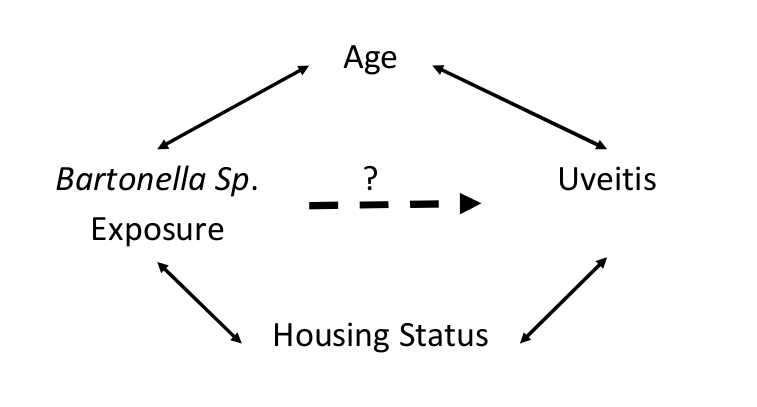
\includegraphics[scale=0.3]{figure1.jpg}
	\caption{Flow Diagram showing proposed Biological Rationale for study, including exposure, outcome and covariates }
	\label{fig:1}
\end{figure*}

\begin{figure*}[h!]
	\centering
	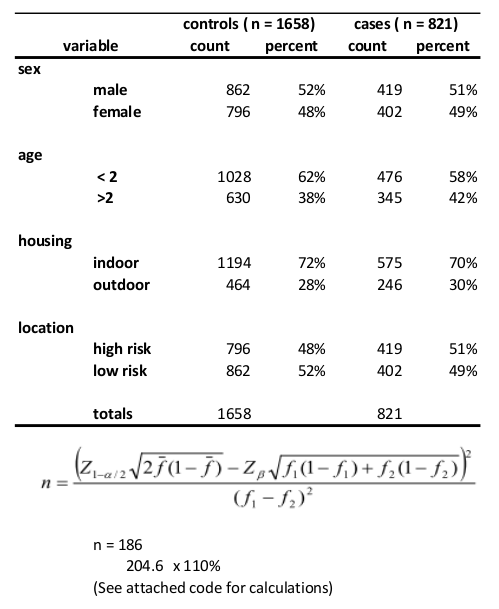
\includegraphics[scale=0.5]{table1.jpg}
	\caption{Characteristics of study participants and sample size calulations.}
	\label{tab:1}
\end{figure*}
 
\begin{figure*}[h!]
	\centering
	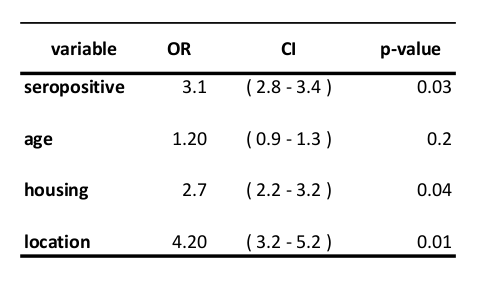
\includegraphics[scale=0.5]{table2.jpg}
	\caption{Odds Ratios (OR) for the association between uveitis and \emph{Bartonella sp.} infection status, age, housing status and geographical location.}
	\label{tab:2}
\end{figure*}

\begin{figure*}[h!]
	\centering
	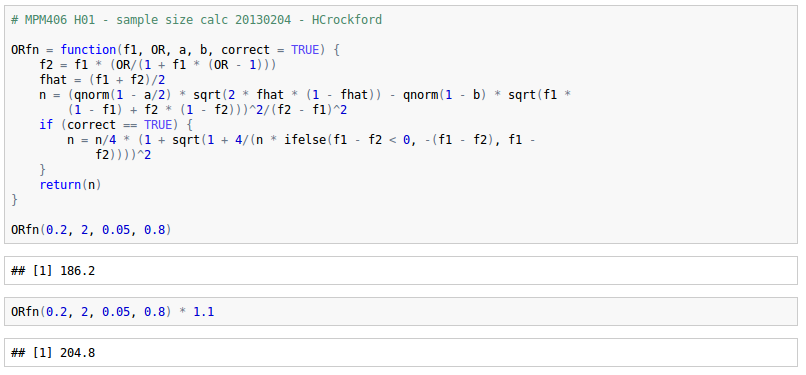
\includegraphics[scale=0.5]{samplesizecalc.jpg}
	\caption{Sample size function and calculation output from R.}
	\label{fig:samplesizecalc}
\end{figure*}

\clearpage
\bibliographystyle{unsrt}
\bibliography{bart.bib}



\end{document}

%%%%%
%% cats admitting to banfield - indoor, looked after, less flea risk.

% need to establish prev in control control group and then establish sample size based on OR you want - (2 - doubling fo risk)

% interactoins - 
%% make streamlined as possible. but need at least one confounder, not necc any interactions, can say did not find any (kim paper for technique - none stat sig so not included). potential effect modify - wualitative. 
% if include need to show OR with and without interactions.
% table 1 - cats in study,. throw in other factors that wont include - make them the same. e.g. age w exposure outcome and not on causal path. - no sig p value. 
% fig 1 - exposure b \emph{Bartonella sp.} , outcome ev.

% diagram bartonella causing uveitis, age associated w bartonella and uveitis (double ended arrow.) then show in table.( anythign in table that same do not need to have in diagram.

% adress in study limitation - only cats that are looked after - findings only apply to this 

% strength - most cats that would be worried about

% summ up - further needed - take to cohort, clinical trial

